\documentclass[{../../master}]{subfiles}
\graphicspath{{../../}}  % 個別コンパイル時の画像パスを解決する

\begin{document}

\section{GMappingのアルゴリズムの概要}
\label{sec:gmapping_algorithm}

GMappingは格子ベースの地図を扱うベイズフィルタ系のSLAMアルゴリズムです.
FastSLAM2.0のアプローチを採用しており,スキャンマッチングによってオドメトリを修正することにより,少ないパーティクルでも良好な推定を行うことができるのが特徴です.

\subsection{GMappingが扱う問題}

ロボットの初期姿勢$\bm{x}_{0}$,観測の時系列リスト$z_{1:t}$,オドメトリ情報$u_{1:t}$が得られたとき,ロボットの軌跡$\bm{x}_{1:t}$と地図$m$の結合確率分布を求めます.
\footnote{論文\cite{Gmapping}に書かれている数式と少し異なりますが,表している事象は同じです.}

\begin{equation}
  p(\bm{x_{1:t}}, m \mid \bm{x}_{0}, z_{1:t}, u_{1:t})
  \label{eq:target_distribution}
\end{equation}

ここで,$\bm{x}_{t}$はロボットの姿勢(Pose)を表すベクトルであり,$\bm{x}_{x} = (x_{t}, y_{t}, \theta_{t})^T$です.
$z_{t}$は時刻$t$で得られた観測の情報で,GMappingではスキャンデータが用いられます.
$u_{t}$は,時刻$t-1$から時刻$t$までにロボットが移動した距離を,ホイールオドメトリで求めた情報です.
また,$1:t$の表記は時刻$1$から時刻$t$までの時系列のリストを表しています.

SLAMの目的は式\ref{eq:target_distribution}の確率分布を求めることにあります.
確率分布を求めることができれば,確率密度が一番高いところにロボットがいるのが尤もらしいと言えるため,結果的にロボットの姿勢を求めることに繋がります.

しかし,式\ref{eq:target_distribution}の確率分布がどのような形状をしているのかは誰にもわかりません.
従って,式\ref{eq:target_distribution}を直接求めることはほぼ不可能に近い難問になります.
そのため,何らかの近似や仮定を用いることによって確率分布を求めることになります.
その近似手法の1つが,GMappingでも用いられているパーティクルフィルタです.

% TODO: パーティクルフィルタの概要の説明.1次元のグラフかなんかを書いて説明する

GMappingではRao-Blackwellizationと呼ばれる因数分解を適用して,式\ref{eq:target_distribution}の確率分布を分解しています.

\begin{equation}
  \begin{split}
    &p(\bm{x_{1:t}}, m \mid \bm{x}_{0}, z_{1:t}, u_{1:t}) \\
    &= p(m \mid \bm{x}_{1:t}, \bm{x}_{0}, u_{1:t}, z_{1:t}) \cdot p(\bm{x}_{1:t} \mid \bm{x}_{0}, u_{1:t}, z_{1:t}) \\
    &= p(m \mid \bm{x}_{0:t}, z_{1:t}) \cdot p(\bm{x}_{1:t} \mid z_{1:t}, u_{1:t})
  \end{split}
  \label{eq:rao_blackwellized_distribution}
\end{equation}

式\ref{eq:target_distribution}にRao-Blackwellizationを適用したのが式\ref{eq:target_distribution}です.
式\ref{eq:rao_blackwellized_distribution}を見ると,この問題はロボットの姿勢の分布$p(\bm{x}_{1:t} \mid z_{1:t}, u_{1:t})$を求める問題と,地図$p(m \mid \bm{x}_{0:t}, z_{1:t})$を求める問題に分解して考えられるようになります.

\subsection{地図の表現形式}

ROSにおける占有格子地図の形式は\textsf{nav\_msgs/OccupancyGrid}\footnote{\url{http://docs.ros.org/en/melodic/api/nav_msgs/html/msg/OccupancyGrid.html}}で定義されています.
コード\ref{code:occupancy_grid_definition}にメッセージの定義を引用します.

\begin{lstlisting}[label=code:occupancy_grid_definition, caption=Message Difinition of \textsf{nav\_msgs/OccupancyGrid}]
# This represents a 2-D grid map, in which each cell represents the probability of
# occupancy.

Header header 

#MetaData for the map
MapMetaData info

# The map data, in row-major order, starting with (0,0).  Occupancy
# probabilities are in the range [0,100].  Unknown is -1.
int8[] data
\end{lstlisting}

\textsf{nav\_msgs/OccupancyGrid}は地図のメタデータとセルのデータを持ちます.

メタデータは\textsf{nav\_msgs/MapMetaData}\footnote{\url{http://docs.ros.org/en/melodic/api/nav_msgs/html/msg/MapMetaData.html}}で定義されています.
コード\ref{code:map_metadata_definition}にメタデータの定義を引用します.

\begin{lstlisting}[label=code:map_metadata_definition, caption=Message Definition of \textsf{nav\_msgs/MapMetaData}]
# This hold basic information about the characterists of the OccupancyGrid

# The time at which the map was loaded
time map_load_time
# The map resolution [m/cell]
float32 resolution
# Map width [cells]
uint32 width
# Map height [cells]
uint32 height
# The origin of the map [m, m, rad].  This is the real-world pose of the
# cell (0,0) in the map.
geometry_msgs/Pose origin
\end{lstlisting}

地図は1つのセルが-1から100までの数値を取る2次元のマトリクスとして定義され,そのデータは行優先順(Row-Major Order)で1次元配列として保存されます.

\begin{equation}
  m_{t} = [m_{t, 0}, m_{t, 1},  \ldots, m_{t, N}]
\end{equation}

地図の幅及び高さはメタデータ内の\textsf{width},\textsf{height}にそれぞれ記録されます.
セルの原点[0, 0]であり,地図の一番左下にあります.
このセルの原点[0, 0]が,グローバル座標系のどの位置,どの角度に対応するかを示すのが,メタデータ内の\textsf{origin}です.
地図が更新されてサイズが大きくなったとき,この\textsf{origin}と\textsf{width},\textsf{height}を更新することで,1次元配列で2次元地図を表現しています.

セルの値が$-1$のとき未知の領域,$0$のとき自由領域,$100$のとき障害物領域を示します.
障害物がある確率に従って0から100までの値を取ります.

\subsection{レーザースキャンの表現形式}

ROSにおけるレーザースキャンの形式は\textsf{sensor\_msgs/LaserScan}\footnote{\url{http://docs.ros.org/en/api/sensor_msgs/html/msg/LaserScan.html}}で定義されています.
コード\ref{code:laserscan_definition}にメッセージの定義を引用します.

\begin{lstlisting}[label=code:laserscan_definition, caption=Message Definition of \textsf{sensor\_msgs/LaserScan}]
# Single scan from a planar laser range-finder
#
# If you have another ranging device with different behavior (e.g. a sonar
# array), please find or create a different message, since applications
# will make fairly laser-specific assumptions about this data

Header header            # timestamp in the header is the acquisition time of 
                          # the first ray in the scan.
                          #
                          # in frame frame_id, angles are measured around 
                          # the positive Z axis (counterclockwise, if Z is up)
                          # with zero angle being forward along the x axis
                          
float32 angle_min        # start angle of the scan [rad]
float32 angle_max        # end angle of the scan [rad]
float32 angle_increment  # angular distance between measurements [rad]

float32 time_increment   # time between measurements [seconds] - if your scanner
                          # is moving, this will be used in interpolating position
                          # of 3d points
float32 scan_time        # time between scans [seconds]

float32 range_min        # minimum range value [m]
float32 range_max        # maximum range value [m]

float32[] ranges         # range data [m] (Note: values < range_min or > range_max should be discarded)
float32[] intensities    # intensity data [device-specific units].  If your
                          # device does not provide intensities, please leave
                          # the array empty.
\end{lstlisting}

レーザースキャンの各距離データは1次元配列に格納されています.

\begin{figure}[ht]
  \centering
  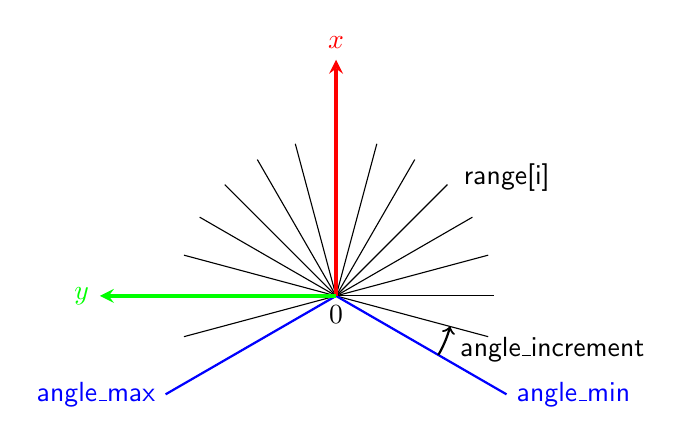
\begin{tikzpicture}
    %\draw[help lines, step=0.5] (-3, -3) grid (3, 3);
    
    % Range
    \foreach \r in {-120, -105, ..., 120}
      \draw[rotate around={\r: (0, 0)}] (0, 0) -- (0, 2);
    
    \draw (1.5, 1.5) node[right]{\textsf{range[i]}};

    \draw[blue, thick, rotate around={-120: (0, 0)}] (0, 0) -- (0, 2.5) node[right]{\textsf{angle\_min}};
    \draw[blue, thick, rotate around={120: (0, 0)}] (0, 0) -- (0, 2.5) node[left]{\textsf{angle\_max}};

    % Origin
    \draw (0, 0) node[below]{0};
    % X Axis
    \draw[->, >=stealth, very thick, red] (0, 0) -- (0, 3) node[above]{$x$};
    % Y Axis
    \draw[->, >=stealth, very thick, green] (0, 0) -- (-3, 0) node[left]{$y$};

    \draw[thick, ->, rotate around={-30: (0, 0)}] (1.5, 0) arc [start angle=0, delta angle=15, radius=1.5] node[below right]{\textsf{angle\_increment}};
  \end{tikzpicture}
  \caption{\textsf{sensor\_msgs/LaserScan}}
  \label{fig:sensor_msgs_laserscan}
\end{figure}

\subsection{オドメトリ状態遷移モデル}

\subsection{レーザービームの尤度場モデル}

\subsection{リサンプリングアルゴリズム}

\end{document}